\documentclass[mathserif,handout]{beamer}
%\documentclass{beamer}
\usetheme{Warsaw}
\usecolortheme{seahorse}
\usecolortheme{orchid}
\usepackage{amsmath,verbatim}
\usepackage{listings}
\usepackage[english]{babel}
\usepackage{movie15}
\setbeamercovered{transparent}

\newcommand{\Deltap}{\ensuremath{\Delta^{\!+}}}
\newcommand{\trans}{\ensuremath{{}^\mathrm{T}}}
\newcommand{\eps}{\varepsilon}
\newcommand*{\approxdist}{\mathrel{\vcenter{\offinterlineskip
\vskip-.25ex\hbox{\hskip.55ex$\cdot$}\vskip-.25ex\hbox{$\sim$}
\vskip-.5ex\hbox{\hskip.55ex$\cdot$}}}}

\lstdefinelanguage{myR}
{
   language=R,
   otherkeywords={read.table, set.seed, head},
   deletekeywords={url,codes, t, dt, Call, formula,Q, R, on,by,hat,is,
col, set,start,end,deltat,zip},
   sensitive=true,
   breaklines=true,
   morecomment=[l]{\#},
   morestring=[b]",
   morestring=[b]',
   basicstyle =\ttfamily\small,
   keywordstyle=\bfseries,
   showtabs=false,
   showstringspaces=false,
   literate= {~}{$\sim$}{2},
   numberstyle=\sffamily\scriptsize,
   stepnumber=2
 }


\begin{document}

\title{Parallelisation strategies for Monte Carlo algorithms}
\author[Darren Wilkinson --- BIRS, Banff, Canada, 6/3/14]{\textbf{\large Darren Wilkinson} \\
\alert{\url{http://tinyurl.com/darrenjw}}\\
School of Mathematics \& Statistics\\Newcastle University, UK}
\date{BIRS Workshop on Scalable Bayesian Computation,\\BIRS, Banff, Canada, 6th March 2014}

\frame{\titlepage}


\frame{
\frametitle{Outline}
\begin{itemize}
\item Monte Carlo
\item PRNG and PPRNG
\item MCMC (parallel chains and parallelised single chains)
\item Case study: SV Models
\item ABC (and ABC-SMC)
\item Parallel particle filtering and pMCMC
\item Hybrid algorithms
\item Functional programming, immutable data structures and parallelisation
\item Summary
\end{itemize}
\vspace{1ex}

}


\section{Monte Carlo and Markov chain Monte Carlo}

\subsection{Monte Carlo}

\frame{
\frametitle{Monte Carlo}
\begin{itemize}
\item
\(
\displaystyle
\phi \sim \Pi \text{ and } \Pi \text{ has density } \pi(\phi)
\)
\item
\(
\displaystyle
I  = E_\Pi(t(\phi)) = \int t(\phi)d\Pi(\phi) = \int t(\phi)\pi(\phi)d\phi
\)
\item
\[
I \simeq \frac{1}{n} \sum_{i=1}^n t(\phi^{(i)})
\]
where $\phi^{(i)} \sim \Pi,\ i=1,2,\ldots n$.
\item
Very easy to parallelise! 
\item Suppose we have $N$ processors, where
$N|n$...
\end{itemize}
}

\frame{
\frametitle{Parallel Monte Carlo integral}
\begin{enumerate}
\item Master program computes $m=n/N$, and passes $m$ to each 
	available processor
\item Each processor ($k$):
	\begin{enumerate}
	\item simulates $m$ independent realisations of $\phi$
	\item computes $S_k = \sum_{i=1}^m t(\phi^{(i)})$
	\item passes $S_k$ back to master program
	\end{enumerate}
\item Master program collects and sums the $S_k$ to give final sum
$S$.
\item Master program returns $S/n$
\end{enumerate}
Need to be careful about independence of random numbers across
processors --- need to understand how PRNG works...
}

\subsection{Parallel pseudo-random number generation}

\frame{
\frametitle{PRNG: pseudo-random number generation}

How does it work?

\setlength{\unitlength}{0.8cm}
\begin{picture}(12,5)
\put(0,2.5){$S_0$}
\put(2,2.5){$S_1$}
\put(4,2.5){$S_2$}
\put(10,2.5){$S_{i-1}$}
\put(12,2.5){$S_i$}
\multiput(0.6,2.68)(2,0){6}{\vector(1,0){1.3}}
\multiput(1.1,2.9)(2,0){6}{$\psi$}
\multiput(2.2,2.3)(2,0){6}{\vector(0,-1){1.3}}
\multiput(2.3,1.7)(2,0){6}{$\rho$}
\put(2,0.5){$u_1$}
\put(4,0.5){$u_2$}
\put(10,0.5){$u_{i-1}$}
\put(12,0.5){$u_i$}
\put(0.1,4.5){$s$}
\put(0.2,4.4){\vector(0,-1){1.5}}
\put(0.3,3.6){$\omega$}
\end{picture}

Actually a big loop (circle), as the state has finite size, and
therefore must eventually return to the original state and cycle.
}


\frame{
\frametitle{PPRNG: parallel pseudo-random number generation}
Problems with multiple processors:
\begin{itemize}
\item Can't share a single stream (too much overhead)
\item Can't use identical streams
\item ``Different seeds'' doesn't completely solve the problem
	\begin{itemize}
	\item this just starts you on a different part of the state
``loop'' --- danger of overlapping streams if seeding is not
sophisticated or simulation is large
	\end{itemize}	
\item Need independent streams on each processor...
	\begin{itemize}
	\item ie. want states to lie on a toroidal lattice rather than
a circular lattice
	\end{itemize}
\end{itemize}
}

\frame{
\frametitle{PPRNG mappings}
\setlength{\unitlength}{0.6cm}
\begin{center}
\begin{picture}(12,12)
\newsavebox{\onestream}
\savebox{\onestream}(12,3.5)[bl]{
\put(0,2.5){$S_0$}
\put(2,2.5){$S_1$}
\put(4,2.5){$S_2$}
\put(10,2.5){$S_{i-1}$}
\put(12,2.5){$S_i$}
\multiput(0.6,2.68)(2,0){6}{\vector(1,0){1.3}}
\multiput(1.1,2.9)(2,0){6}{$\psi$}
\multiput(2.2,2.3)(2,0){6}{\vector(0,-1){1.3}}
\multiput(2.3,1.7)(2,0){6}{$\rho$}
\put(2,0.5){$u_1$}
\put(4,0.5){$u_2$}
\put(10,0.5){$u_{i-1}$}
\put(12,0.5){$u_i$}
}
\put(1,0){\usebox{\onestream}}
\put(1,4){\usebox{\onestream}}
\put(1,8){\usebox{\onestream}}
\multiput(1.3,2.8)(2,0){3}{\scriptsize$3$}
\multiput(11.3,2.8)(2,0){2}{\scriptsize$3$}
\multiput(1.3,6.8)(2,0){3}{\scriptsize$2$}
\multiput(11.3,6.8)(2,0){2}{\scriptsize$2$}
\multiput(1.3,10.8)(2,0){3}{\scriptsize$1$}
\multiput(11.3,10.8)(2,0){2}{\scriptsize$1$}
\multiput(3.25,0.7)(2,0){2}{\scriptsize$3$}
\multiput(11.25,0.7)(2,0){2}{\scriptsize$3$}
\multiput(3.25,4.7)(2,0){2}{\scriptsize$2$}
\multiput(11.25,4.7)(2,0){2}{\scriptsize$2$}
\multiput(3.25,8.7)(2,0){2}{\scriptsize$1$}
\multiput(11.25,8.7)(2,0){2}{\scriptsize$1$}
\put(-1,6.5){$s$}
\put(-0.6,6.7){\vector(1,0){1.5}}
\put(-0.7,7.0){\vector(1,2){1.6}}
\put(-0.7,6.4){\vector(1,-2){1.6}}
\put(0,6.8){$\omega^2$}
\put(-0.3,8.8){$\omega^1$}
\put(-0.5,4.8){$\omega^3$}
\end{picture}
\end{center}
}


\frame{
\frametitle{Example Monte Carlo Integral}

Consider numerical evaluation of the integral
\[
I = \int_0^1 \exp\{-u^2\} du = E_U(\exp\{-U^2\}) \simeq \frac{1}{n}
\sum_{i=1}^n \exp\{-u_i^2\}
\]
where
\[
u_i \sim U(0,1).
\]
}

%\frame{
\begin{frame}[fragile]
\frametitle{Parallel Monte Carlo integral (C+MPI+SPRNG)}
% monte-carlo.c
{\scriptsize
\begin{lstlisting}[language=C]
int main(int argc,char *argv[])
{
  int i,k,N; double u,ksum,Nsum; gsl_rng *r;
  MPI_Init(&argc,&argv);
  MPI_Comm_size(MPI_COMM_WORLD,&N);
  MPI_Comm_rank(MPI_COMM_WORLD,&k);
  r=gsl_rng_alloc(gsl_rng_sprng20);
  for (i=0;i<10000;i++) {
    u = gsl_rng_uniform(r);
    ksum += exp(-u*u);
  }
  MPI_Reduce(&ksum,&Nsum,1,MPI_DOUBLE,MPI_SUM,0,MPI_COMM_WORLD);
  if (k == 0) {
    printf("Monte carlo estimate is %f\n", (Nsum/10000)/N );
  }
  MPI_Finalize();
  exit(EXIT_SUCCESS);
}
\end{lstlisting}
}
\end{frame}
%}

\subsection{Parallel MCMC}

\frame{
\frametitle{MCMC: Parallel chains}

Multiple parallel chains is really easy...
\vspace*{0.8ex}

\textbf{\large Example}

\begin{itemize}
\item Metropolis-Hastings for a standard normal random quantity based on
$U(-\alpha,\alpha)$ innovations.
\item So if chain is currently at $x$, a new candidate $x^\star$ is
simulated from $U(x-\alpha,x+\alpha)$, and this candidate is accepted
with probability $\min\{1,A\}$, where
\[
A  = \phi(x^\star) / \phi(x)
\]
and $\phi(\cdot)$ is the standard normal density.
\end{itemize}
}

%\frame{
\begin{frame}[fragile]
\frametitle{Independent parallel MCMC chains}
% mcmc.c
{\scriptsize
\begin{lstlisting}[language=C]
#include <gsl/gsl_rng.h>
#include "gsl-sprng.h"
#include <gsl/gsl_randist.h>
#include <mpi.h>

int main(int argc,char *argv[])
{
  int k,i,iters; double x,can,a,alpha; gsl_rng *r;
  FILE *s; char filename[15];
  MPI_Init(&argc,&argv);
  MPI_Comm_rank(MPI_COMM_WORLD,&k);
  if ((argc != 3)) {
    if (k == 0)
      fprintf(stderr,"Usage: %s <iters> <alpha>\n",argv[0]);
    MPI_Finalize(); return(EXIT_FAILURE);
  }
  iters=atoi(argv[1]); alpha=atof(argv[2]);
  r=gsl_rng_alloc(gsl_rng_sprng20);
\end{lstlisting}
}
\end{frame}

\begin{frame}[fragile]
\frametitle{ctd.}
{\scriptsize
\begin{lstlisting}[language=C]
  sprintf(filename,"chain-%03d.tab",k);
  s=fopen(filename,"w");
  if (s==NULL) {
    perror("Failed open");
    MPI_Finalize(); return(EXIT_FAILURE);
  }
  x = gsl_ran_flat(r,-20,20);
  fprintf(s,"Iter X\n");
  for (i=0;i<iters;i++) {
    can = x + gsl_ran_flat(r,-alpha,alpha);
    a = gsl_ran_ugaussian_pdf(can) / gsl_ran_ugaussian_pdf(x);
    if (gsl_rng_uniform(r) < a)
      x = can;
    fprintf(s,"%d %f\n",i,x);
  }
  fclose(s);
  MPI_Finalize(); return(EXIT_SUCCESS);
}
\end{lstlisting}
}
\end{frame}
%}

\frame{
\frametitle{Parallel chains MCMC}
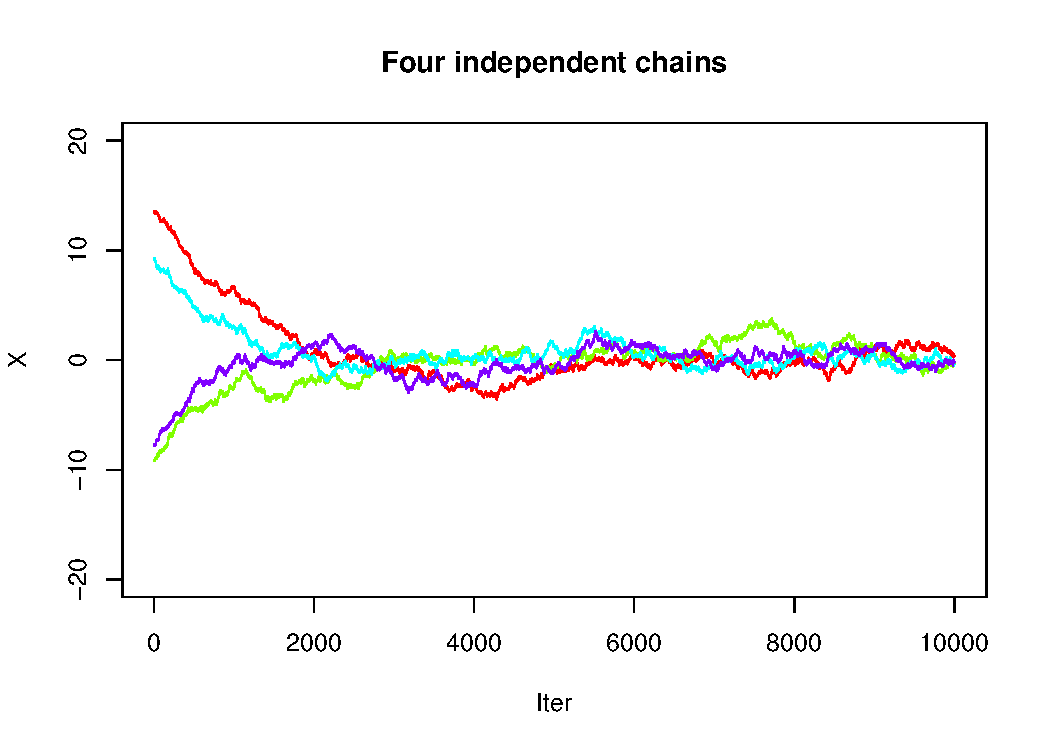
\includegraphics[width=\textwidth]{mcmc-trace}
}

\frame{
\frametitle{Burn-in and speed-up with parallel chains}

\begin{itemize}
\item
If burn-in is $b$ and $n$ iterations are required for the monitoring
run, then
\end{itemize}
\begin{block}{Speed-up}
\[
SpeedUp(N) = \frac{b+n}{b+\frac{n}{N}} \longrightarrow \frac{b+n}{b}
\]
\end{block}
\begin{itemize}
\item
So speed-up is bounded as the number of processors tends to infinity!
\item This is essentially \alert{Amdahl's law} for parallel chains
MCMC...
\end{itemize}
}

\frame{
\frametitle{Parallel chains speed-up for $n=10b$}
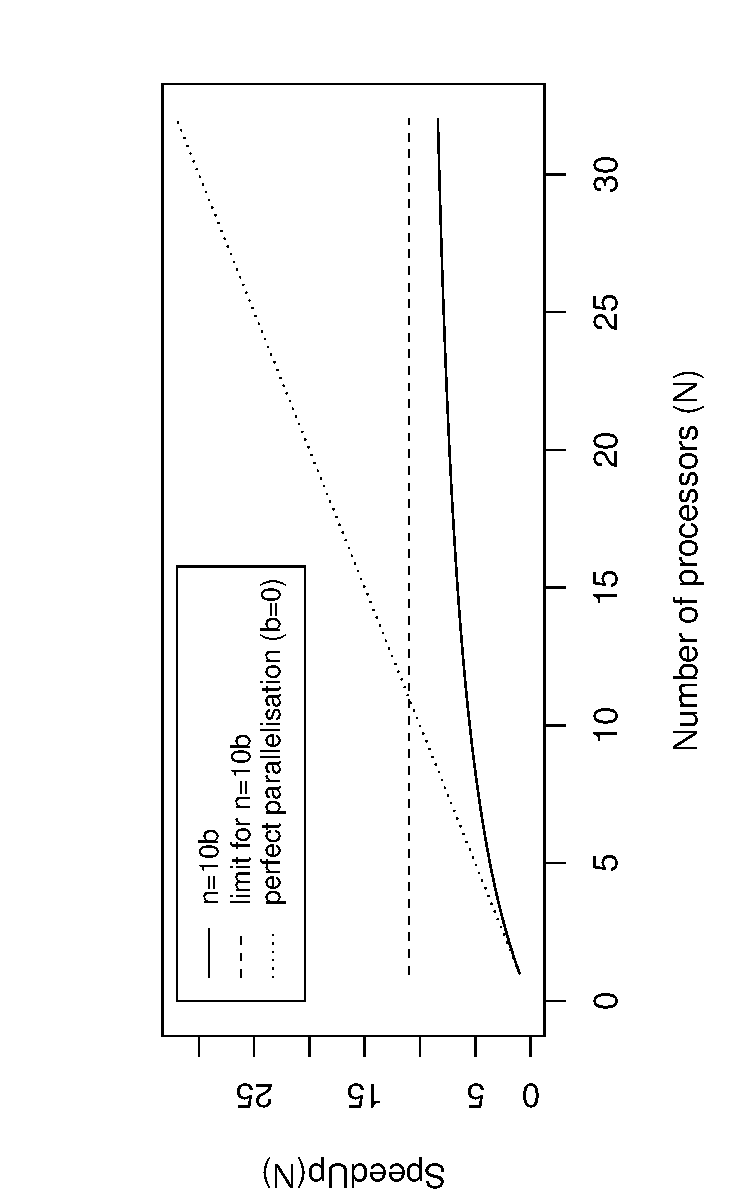
\includegraphics[width=0.6\textwidth,angle=270]{speedup}
}

\frame{
\frametitle{Parallelising single chains}
\begin{itemize}
\item The problem with parallelising MCMC chains is that each proposed
new state depends on the previous state, essentially making it
difficult to farm out multiple iterations to different processors
\item A couple of exceptions:
	\begin{itemize}
	\item For a Metropolis \alert{independence}
	sampler where the evaluation of the likelihood of the proposal
	is time consuming, it is possible to generate many candidates
	and evaluate likelihoods on multiple processors
	\item
	\alert{pre-fetching}: given a (single-block, or random sweep) M-H
	algorithm, can farm out all $2^n$ likelihood evaluations which
	might be required in order to advance the chain by $n$ steps
	(but speedup is only logarithmic in number of processors)
	\end{itemize}
\item Otherwise need to parallelise each iteration...
\end{itemize}
}

\frame{
\frametitle{Parallelised single chain}
Exploit conditional independence...
\begin{itemize}
\item
\(
\pi(\sigma,\theta,y) = \pi(\sigma)\pi(\theta|\sigma)p(y|\sigma,\theta)
\)
\item
\(
\sigma=(\sigma_1,\ldots,\sigma_p),\quad \theta=(\theta_1,\ldots,\theta_q)
\)
\item
Update of $\sigma$ is fast. 
\item Update of $\theta$ is slow. 
\item Parallelise
update of $\theta$.
\item
Simplest case: $\theta_i \perp\hspace{-0.8ex}\perp \theta_j |\sigma,y$
\end{itemize}
}

\frame{
\frametitle{Basic algorithm}
\begin{enumerate}
\item Each processor ($k$):
	\begin{enumerate}
	\item sequentially updates the $q_k$ $\theta$s that have been
assigned to it, using the current value of $\sigma$
	\item computes summary statistics for the new $\theta$s that
will be required to update $\sigma$
	\item passes the summary statistics back to the root process
(master program)
	\end{enumerate}
\item The root process combines the summary statistics in order to
obtain an explicit form for the updating of $\sigma$
\item A new $\sigma$ is sampled and output
\item The new $\sigma$ is distributed out to each process
\end{enumerate}
}

\frame{
\frametitle{Serial dependence}

\begin{block}{Markov dependence}
\[
\theta_i \perp\hspace{-0.8ex}\perp
\theta_j|\theta_{i-1},\theta_{i+1},\sigma,y,\quad j\not= i
\]
\end{block}
\setlength{\unitlength}{0.8cm}
\begin{picture}(13,2)
\multiput(1,1)(2,0){6}{\circle{1}}
\multiput(1.5,1)(2,0){6}{\line(1,0){1}}
\put(0.9,0.9){$\theta_1$}
\put(2.9,0.9){$\theta_2$}
\put(4.9,0.9){$\theta_3$}
\put(6.9,0.9){$\theta_4$}
\put(8.9,0.9){$\theta_5$}
\put(10.9,0.9){$\theta_6$}
\end{picture}
\begin{itemize}
\item
Note that the ``odd'' numbered blocks are conditionally independent of
one another given the ``even'' numbered blocks, and vice versa.
\end{itemize}
}

\frame{
\frametitle{MRF example}
\setlength{\unitlength}{0.8cm}
\begin{picture}(13,9)
\multiput(1,1)(2,0){6}{\circle{1}}
\multiput(1.5,1)(2,0){6}{\line(1,0){1}}
\multiput(1,1.5)(2,0){6}{\line(0,1){1}}
\multiput(1,3)(2,0){6}{\circle{1}}
\multiput(1.5,3)(2,0){6}{\line(1,0){1}}
\multiput(1,3.5)(2,0){6}{\line(0,1){1}}
\multiput(1,5)(2,0){6}{\circle{1}}
\multiput(1.5,5)(2,0){6}{\line(1,0){1}}
\multiput(1,5.5)(2,0){6}{\line(0,1){1}}
\multiput(1,7)(2,0){6}{\circle{1}}
\multiput(1.5,7)(2,0){6}{\line(1,0){1}}
\multiput(1,7.5)(2,0){6}{\line(0,1){1}}
\multiput(1,1)(4,0){3}{\circle*{0.3}}
\multiput(3,3)(4,0){3}{\circle*{0.3}}
\multiput(1,5)(4,0){3}{\circle*{0.3}}
\multiput(3,7)(4,0){3}{\circle*{0.3}}
\end{picture}
}

\frame{
\frametitle{General dependence structures}
\begin{itemize}
\item
Need to divide up the blocks of $\theta$ into sets of blocks which are
conditionally independent, and hence can be updated in parallel.
\item
$T=\{T_1,\ldots,T_c\}$ is a \alert{partition} of
$\{\theta_1,\ldots,\theta_q\}$ where each $T_i$ is a set of blocks
that are conditionally independent given all remaining blocks (and
$\sigma$ and $y$). 
\item
The smallest $c$ for which this is possible is known as the
\alert{chromatic} number of the graph. Finding this number and a
suitable partition is the \alert{graph colouring problem} --- NP hard
in general.
\end{itemize}
}

\frame{
\frametitle{General algorithm}

\begin{enumerate}
\item Each processor ($k$):
	\begin{enumerate}
	\item For each $i$ in 1 to $c$:
		\begin{enumerate}
		\item sequentially updates all the blocks in $T_i$ 
			allocated to it
		\item distributes necessary state information
regarding updates to adjacent processors
		\item receives such information from adjacent processors
		\end{enumerate}
	\item computes summary statistics for the new $\theta$s that
will be required to update $\sigma$
	\item passes the summary statistics back to the root process
(master program)
	\end{enumerate}
\item the root process combines the summary statistics in order to
obtain an explicit form for the updating of $\sigma$
\item a new $\sigma$ is sampled and output
\item the new $\sigma$ is distributed out to each process
\end{enumerate}
}

\frame{
\frametitle{When elements of $\sigma$ are not CI:}

\begin{enumerate}
\item Each processor ($k$):
	\begin{enumerate}
	\item for each $i$ in 1 to $c$:
		\begin{enumerate}
		\item sequentially updates all the blocks in $T_i$ 
			allocated to it
		\item distributes necessary state information
regarding updates to adjacent processors
		\item receives such information from adjacent processors
		\end{enumerate}
	\end{enumerate}
\item for each $i$ in 1 to $p$:
	\begin{enumerate}
	\item each processor (k):
		\begin{enumerate}
		\item computes summary statistics that
will be required to update $\sigma_i$
		\item passes the summary statistics back to the root process
		\end{enumerate}
	\item the root process combines the summary statistics in order to
obtain an explicit form for the updating of $\sigma_i$
	\item a new $\sigma_i$ is sampled and output
	\item the new $\sigma_i$ is distributed out to each processor
	\end{enumerate}
\end{enumerate}
}

\subsection{Case study}

\frame{
\frametitle{Case study: SV models}

\begin{block}{Stochastic volatility model}
\begin{align*}
y_t &= \varepsilon_t\exp\{\alpha_t/2\}, \\
\alpha_t &= \mu + \phi(\alpha_t-\mu) + \eta_t,\quad t=1,2,\ldots,n \\
\varepsilon_t &\sim N(0,1),\quad \eta_t \sim N(0,\sigma_\eta^2)
\end{align*}
\end{block}
\begin{itemize}
\item
Can re-write first equation as
\[
\log y_t^2 = \alpha_t + \log(\varepsilon_t^2)
\]
\item
Use approximation $\log(\varepsilon_t^2) \sim N(-1.27,\pi^2/2)$ to get
a DLM.
\item
Basic idea: divide $\alpha$s up into blocks. Propose update for each
block using a sample from approximating DLM. Correct approximation
using a Metropolis-Hastings step. 
\end{itemize}
}

\frame{
\frametitle{Parallel updating scheme}

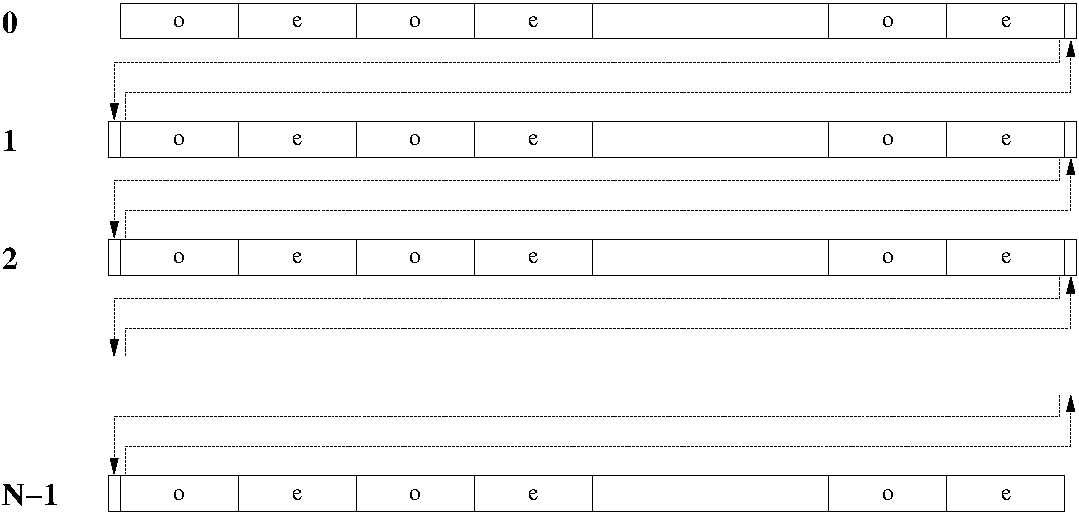
\includegraphics[width=\textwidth]{message}
}

\frame{
\frametitle{MCMC output}
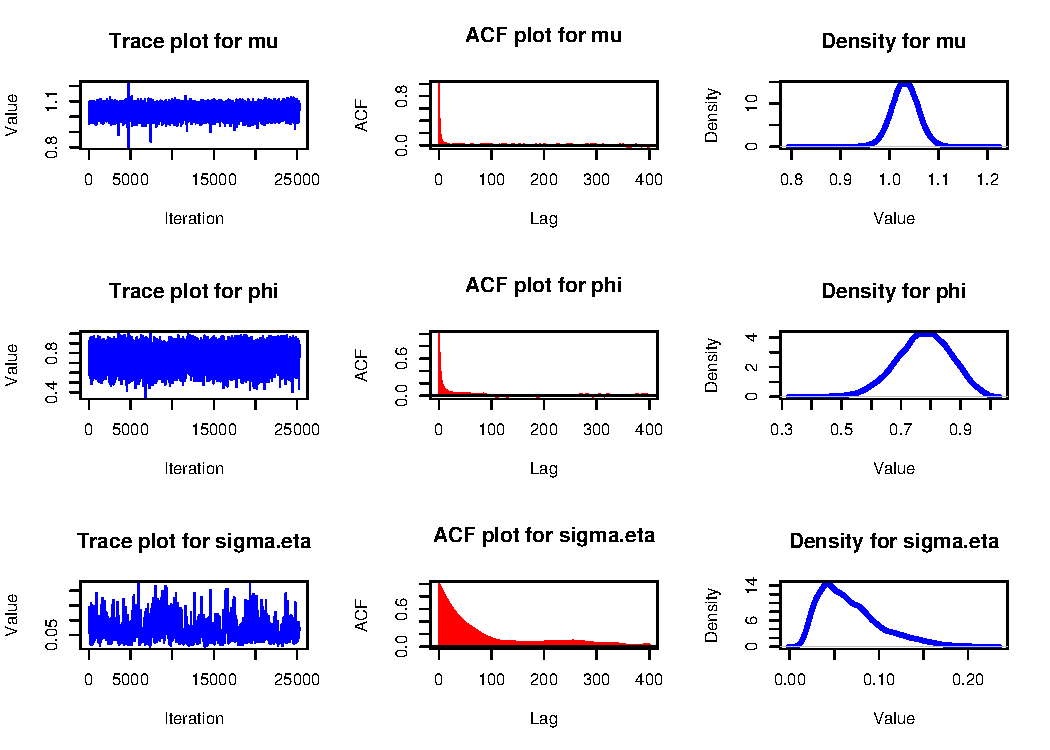
\includegraphics[width=0.9\textwidth]{case-trace}
}

\frame{
\frametitle{Empirical performance}
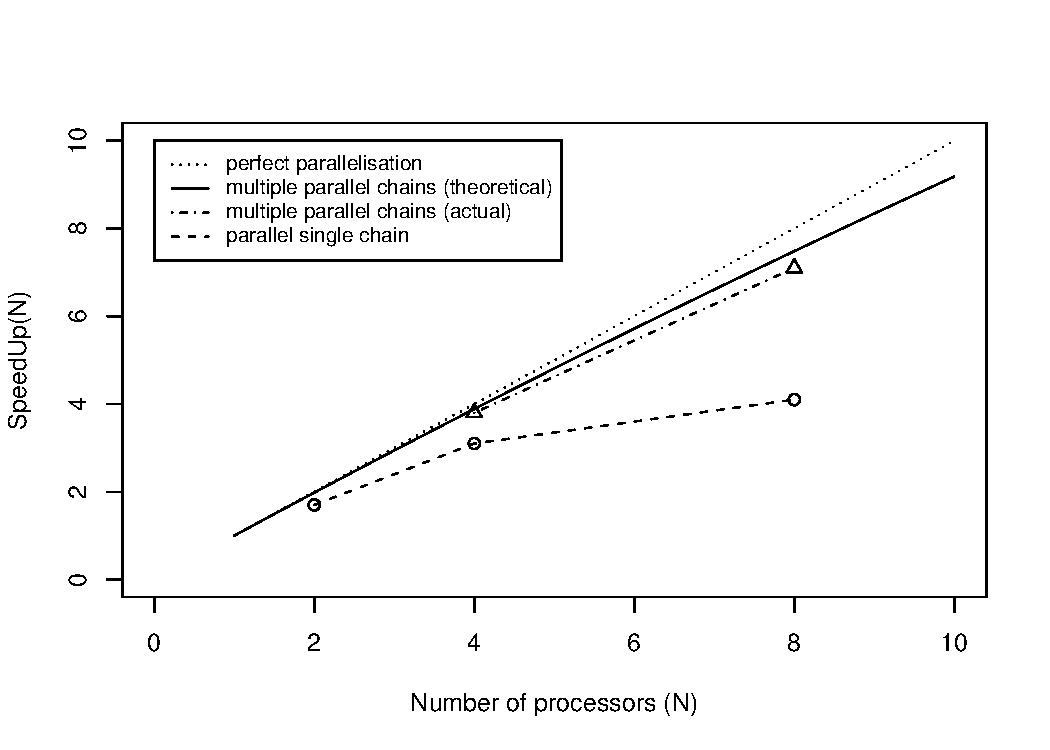
\includegraphics[width=0.9\textwidth]{case-speed}
}

\section{Likelihood free Monte Carlo algorithms}

\subsection{ABC}


\frame{
\frametitle{Alternative: approximate Bayesian computation (ABC)}
\begin{itemize}
\item Since
  $\pi(\theta,\mathbf{x},\mathcal{Y})=\pi(\theta)\pi(\mathbf{x}|\theta)\pi(\mathcal{Y}|\theta,\mathbf{x})$, it is trivial to generate samples from $\pi(\theta,\mathbf{x},\mathcal{Y})$ and to marginalise these down to $\pi(\theta,\mathcal{Y})$ 
\item Exact rejection algorithm: generate
  $(\theta^\star,\mathcal{Y}^\star)$ from $\pi(\theta,\mathcal{Y})$
  and keep provided that $\mathcal{Y}=\mathcal{Y}^\star$ otherwise
  reject and try again
\item This gives exact realisations from $\pi(\theta|\mathcal{Y})$,
  but in practice the acceptance rate will be very small (or zero)
\item ABC: Define a metric on the sample space, $\rho(\cdot,\cdot)$,
  and accept $(\theta^\star,\mathcal{Y}^\star)$ if
  $\rho(\mathcal{Y},\mathcal{Y}^\star)<\eps$
\item  This gives exact realisations from
  $\pi(\theta|\rho(\mathcal{Y},\mathcal{Y}^\star)<\eps)$, which tends
  to the true posterior as $\eps\longrightarrow 0$
\item Still problematic if there is a large discrepancy between the
  prior and posterior...
\end{itemize}
}

\frame{
\frametitle{ABC--SMC}
\begin{itemize}
\item Interest in a Bayesian posterior distribution
\[
\pi(\theta|x) \propto \pi(\theta)f(x|\theta)
\]
where $f(x|\theta)$ is intractable
\item Observed data $x_0$
\item Sequence of approximations
\[
\pi_t(\theta) = \pi(\theta|\rho(x,x_0)<\eps_t),
\]
where $\infty=\eps_0>\eps_1>\cdots>\eps_n>0$ and $\rho(\cdot,\cdot)$
is a suitable metric on data space
\item $\pi_0$ is the prior, and for sufficiently small $\eps_n$,
  hopefully $\pi_n$ not too far from the posterior, $\pi(\theta|x_0)$
\item Progressively reduce tolerances to improve agreement between
  successive distributions and hopefully improve acceptance rates
\end{itemize}
}

\frame{
\frametitle{ABC--SMC algorithm}
\begin{itemize}
\item Suppose we have a large (possibly weighted) sample of size $N$
  from $\pi_{t-1}(\theta)$, $\{\theta_1,\ldots,\theta_N\}$ with
  normalised weights $\tilde{w}_{t-1}^i$
\item Pick $\theta_i^\star \sim \pi_{t-1}(\theta)$ (weighted
  particles)
\item Perturb $\theta_i^{\star\star}\sim
  K(\theta_i^\star,\theta_i^{\star\star})$
\item Simulate $x^\star\sim f(x^\star|\theta^{\star\star})$ from
  intractable likelihood model
\item Accept only if $\rho(x^\star,x_0)<\eps_t$, otherwise reject go back to
  the start and pick another $\theta_i^\star$
\item Keep $\theta^{\star\star}$ as $i$th member of new sample, and
  compute its weight as
\[
w_t^i = \frac{\pi(\theta^{\star\star})}{\sum_{j=1}^N
  \tilde{w}_{t-1}^i K(\theta_j,\theta^{\star\star})}
\]
\item Once a sample of size $N$ is obtained, normalise weights and
  increment $t$
\end{itemize}
Parallelises well, but is approximate.
}

\subsection{pMCMC}

\frame{
\frametitle{Particle marginal Metropolis--Hastings (PMMH)}
\begin{itemize}
\item Use a particle filter to simulate an approximate sample from
  $\pi(\mathbf{x}|\mathcal{Y},\theta)$
\item Correct the acceptance probability to ensure that the target of
  the MCMC scheme is still the exact posterior
  $\pi(\theta,\mathbf{x}|\mathcal{Y})$
\item If a bootstrap particle filter is used, then this relies only on
  the ability to forward simulate from the process, and the entire
  procedure is ``likelihood--free''
\item pMCMC is the only obvious practical option for constructing
  global likelihood--free MCMC algorithms which are exact
  (\alert{Andrieu et al., 2010})
\item See \alert{Golightly \& W (2011)} for applications to POMP models
\end{itemize}
}

\frame{
\frametitle{``Sticking'' and tuning of PMMH}
\begin{itemize}
\item As well as tuning the $\theta$ proposal variance, it is
  necessary to tune the number of particles, $N$ in the particle filter ---
  need enough to prevent the chain from sticking, but computational
  cost roughly linear in $N$
\item
Number of particles necessary depends on $\theta$, but don't know
$\theta$ \emph{a priori}
\item Initialising the sampler is non-trivial, since much of parameter
  space is likely to lead to likelihood estimates that are numerically
  equal to zero --- how to move around when both current and proposed
  values have zero likelihood?!
\item Without careful tuning and initialisation, burn-in, convergence
  and mixing can all be very problematic...
\end{itemize}
}

\frame{
\frametitle{Adaptive ABC--SMC}
\begin{itemize}
\item PMMH algorithms require careful tuning, and are not trivial to
  parallelise 
\item Multiple parallel chains benefit from being initialised at
  samples from the posterior, in order to minimise burn-in
\item Tuning the number of particles to use in the particle filter is
  best done by averaging over a sample from the posterior
\item Adaptive ABC--SMC can be used to generate a sample from an
  approximation to the posterior, which is good enough for tuning and
  initialisation of PMMH chains
  \begin{itemize}
  \item ABC algorithms parallelise well, so this strategy is well
    suited to taking advantage of parallel hardware
  \item ABC--SMC algorithms also require tuning, but reasonable
    default choices work mostly OK for POMP models
  \end{itemize}
\item Multiple independent tuned PMMH chains can then target the exact
  posterior
\end{itemize}
}

\frame{
\frametitle{Comparing adaptive ABC--SMC against pMCMC}
\centerline{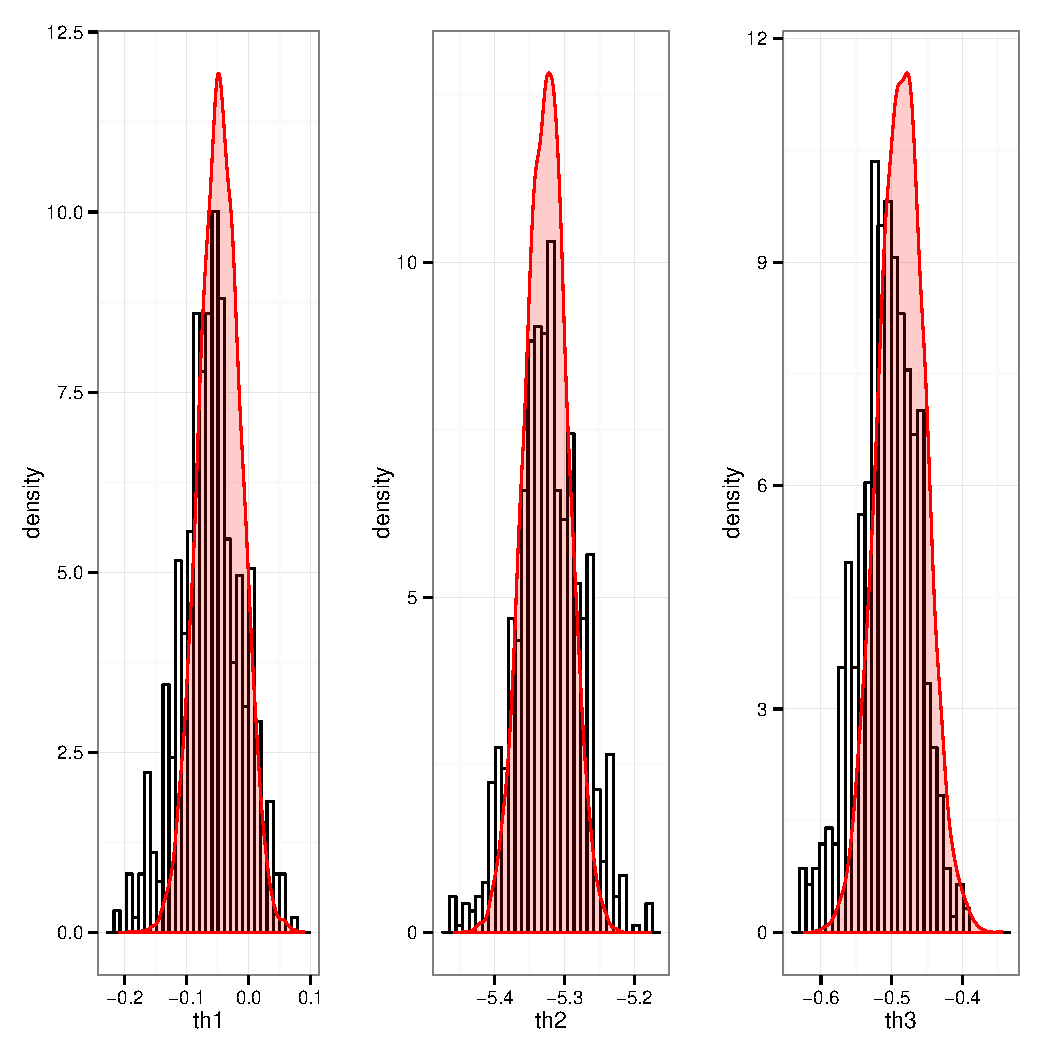
\includegraphics[width=0.6\textwidth]{abcplot}}

Observations on both species with known noise
}

\frame{
\frametitle{PMMH chains}

\centerline{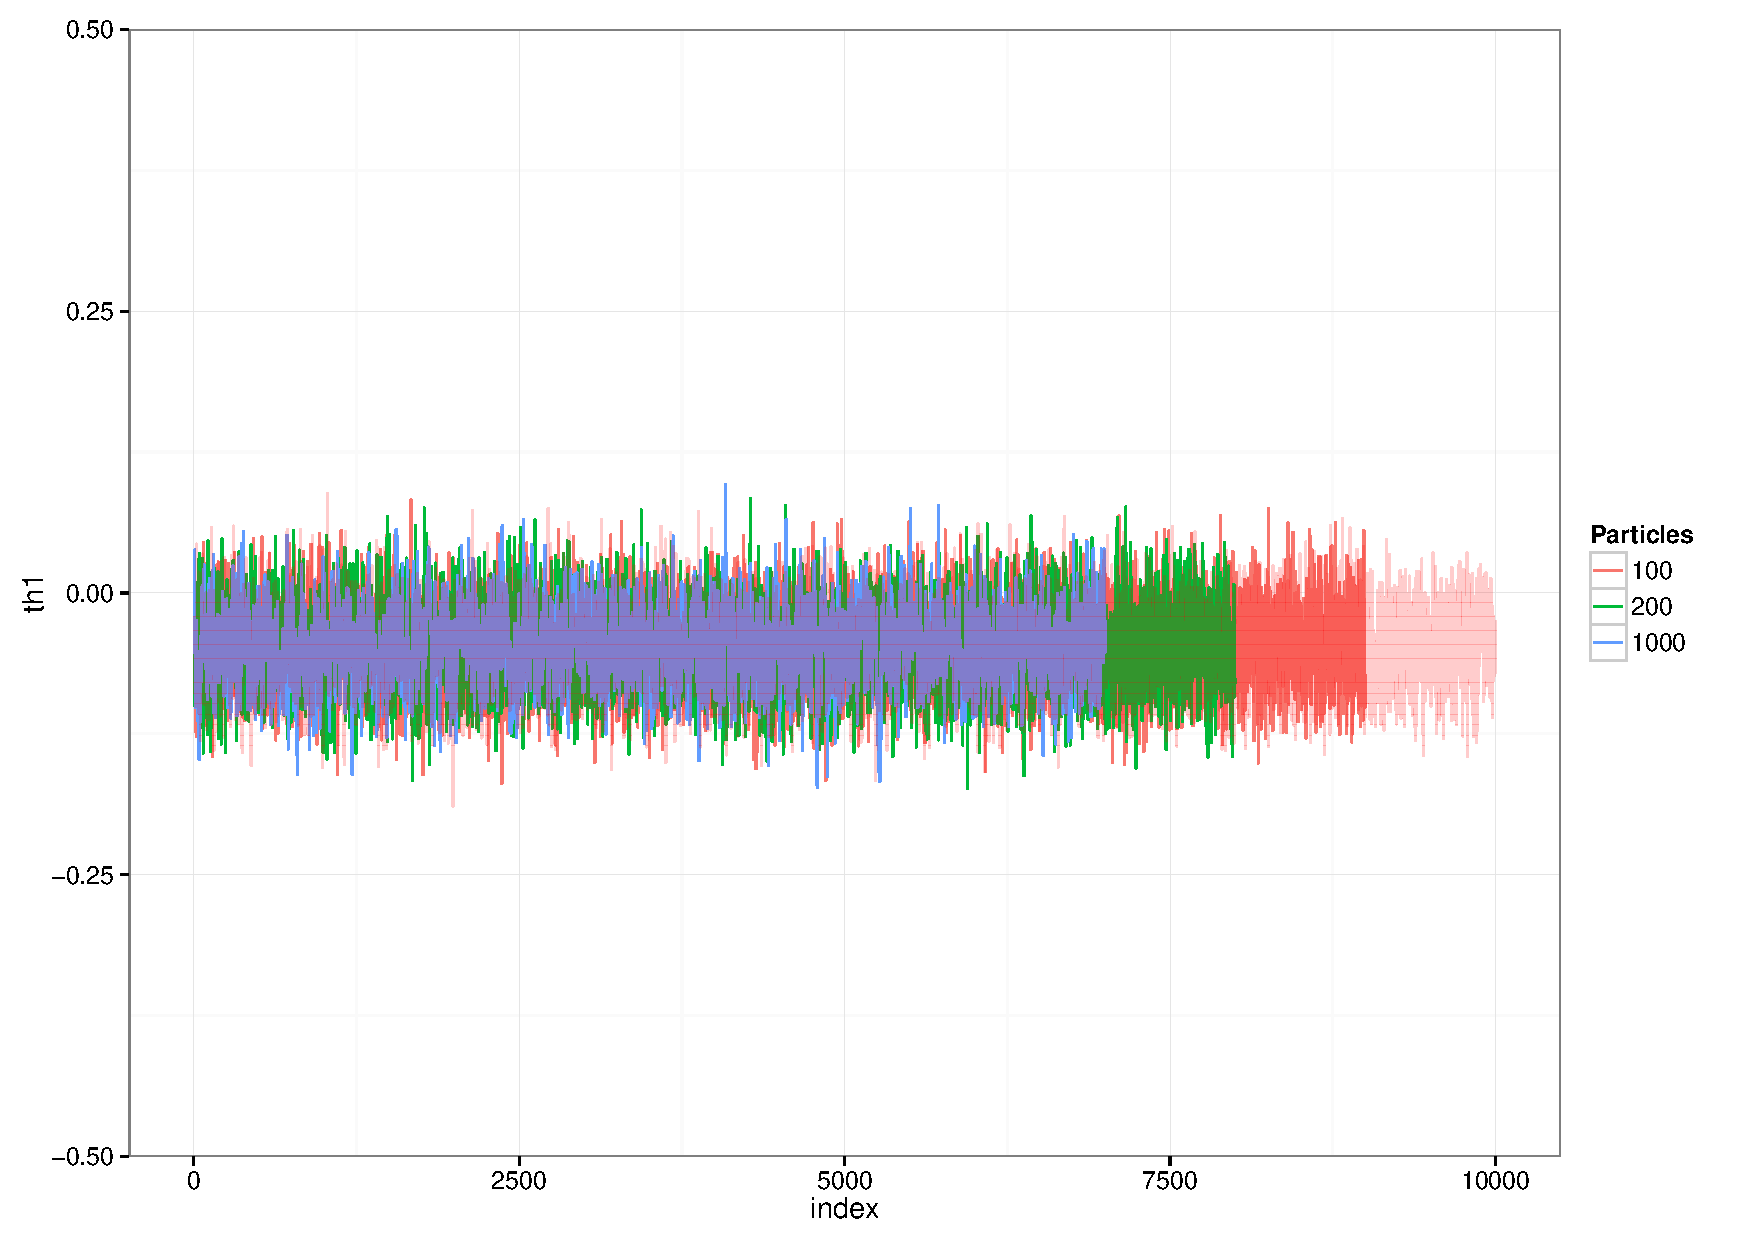
\includegraphics[width=0.8\textwidth]{pmcmcConverganceusingabc}}

PMMH chains initialised using samples from the ABC--SMC posterior (joint work with Jamie Owen and Colin Gillespie)
}

\subsection{SMC}

\frame{
\frametitle{SMC}
\begin{itemize}
\item What's up with parallelising SMC?!
\item I claimed that ABC--SMC parallelises well and that pMCMC doesn't
\item But they both have SMC in the inner loop --- how can that be?!
\item Granularity!
\item In ABC--SMC there will only be a handful of normalisation and resampling steps in total
\item In pMCMC there may be $T$ resampling steps per iteration, and there could be millions of iterations...
\end{itemize}
}

\begin{frame}[fragile]
\frametitle{Parallel particle filter in R}
{\small
\begin{lstlisting}[language=myR]
function(...) {
    xmat = simx0(n, t0, ...)
    ll = 0
    for (i in 1:length(deltas)) {
    xmat=t(sapply(mclapply(split(xmat,row(xmat)), stepFun, t0=times[i], deltat=deltas[i], ...),cbind))
        w = apply(xmat, 1, dataLik, t = times[i + 1], y = data[i,], log = FALSE, ...)
        ll = ll + log(mean(w))
        rows = sample(1:n, n, replace = TRUE, prob = w)
        xmat = xmat[rows, ]
    }
    ll
}
\end{lstlisting}
}
\end{frame}

\section{Functional programming}

\subsection{Functional approach to parallelism}

\frame{
\frametitle{Functional approaches to concurrency and parallelisation}
\begin{itemize}
\item Previous code written a rather functional style --- a function returning a function closure that uses ``map" and ``reduce" operations
\item Not lots of nested ``for" loops and imperative directives working with \alert{shared mutable state} (difficult for concurrency --- locks and synchronisation issues)
\item Functional languages, \alert{immutable state}, and \alert{referentially transparent} (\alert{side-effect} free) declarative workflow patterns are widely used for systems which really need to scale (leads to naturally parallel code)
\item Different sorts of ``scale" including:
  \begin{itemize}
  \item Scaling to big computations for relatively small data (HPC)
  \item Scaling to big models and/or data --- more like distributed computing
  \end{itemize}
\end{itemize}
}

\begin{frame}[fragile]
\frametitle{Parallel Monte Carlo integral in Scala}
{\scriptsize
\begin{lstlisting}[language=java]
object MonteCarlo {
  @tailrec
  def sum(its: Long,acc: Double): Double = {
    if (its==0) 
      (acc)
    else {
      val u=ThreadLocalRandom.current().nextDouble()
      sum(its-1,acc+exp(-u*u))
    }
  }
  def main(args: Array[String]) = {
    val N=args(0).toInt
    val iters=1000000000
    val its=iters/N
    val sums=(1 to N).toList.par map {x => sum(its,0.0)}
    val result=sums.reduce(_+_)
    println(result/iters)
  }
}
\end{lstlisting}
}
Actually runs \alert{faster} than the C+MPI version...
\end{frame}

\subsection{Functors, applicatives, monoids, monads, ...}

\frame{
\frametitle{Category theory}
Dummies guide:
\begin{itemize}
\item A ``collection" (or parametrised ``container" type) together with a ``map" function (defined in a sensible way) represents a \alert{functor}
\item If the collection additionally supports a (sensible) ``apply" operation, it is an \alert{applicative}
\item If the collection additionally supports a (sensible) ``flattening" operation, it is a \alert{monad} (required for composition)
\item For a ``reduce" operation on a collection to parallellise cleanly, the type of the collection together with the reduction operation must define a \alert{monoid} (must be an \alert{associative} operation, so that reductions can proceed in multiple threads in parallel)
\end{itemize}

}

\frame{
\frametitle{Monoids}
\centerline{$x_1+x_2+x_3+x_4=((x_1+x_2)+x_3)+x_4=(x_1+x_2)+(x_3+x_4)$}
\vspace{1ex}

Some examples from this workshop:
\begin{itemize}
\item Summing up (averaging) Monte Carlo samples to estimate an expectation
\item Pooling Monte Carlo samples (including parallel MCMC chains)
\item Consensus Monte Carlo (weighted) summing (averaging) of subsample MCMC chains
\item Adding (averaging) statistical regular paving histogram trees
\item ...
\end{itemize}
Monoids, functors, applicatives and monads provide the mathematical structure which underpins all workflow based split/apply/combine/reduce type strategies to parallelism. 
}

\frame{
\frametitle{Scala ecosystem}
\alert{Scala} --- name derives from ``\emph{Scalable Language}" --- designed for concurrency and parallelism
{\small\begin{itemize}
\item \alert{Akka} --- actor-based concurrency framework (inspired by Erlang)
\item \alert{Spark} --- scalable analytics library, including some ML (from Berkeley AMP Lab)
\item \alert{Algebird} --- abstract algebra (monoid) support library (from Twitter)
\item \alert{Scalding} --- cascading workflow library (from Twitter)
\item \alert{Storm} --- streaming analytics library (from Twitter)
\item \alert{Scalaz} --- category theory types (functors, monads, etc.)
\item \alert{Breeze} --- scientific and numerical library (including nonuniform random number generation and numerical linear algebra)
\item \alert{Saddle} --- data library
\end{itemize}}
Large ecosystem of software libraries and developers using Scala in the big data space...
}

\section{Summary and conclusions}

\subsection{Summary}

\frame{
\frametitle{Summary}
\begin{itemize}
\item Unlike plain Monte Carlo, MCMC is not straightforward to
parallelise
\item For difficult problems with large state spaces, parallelisation
of an MCMC algorithm is possible, using the sparse conditional independence
structure of the underlying statistical model --- but these algorithms
have tight synchronization requirements and tend not to scale very
well as a result
\item Parallel chains MCMC can scale reasonably well so long as burn-in is not significant
\item (Non-MCMC) ABC algorithms parallelise well
\item There are many ways to exploit parallelism, and
statisticians should perhaps look to functional languages and concurrency models, and distributed computing technologies for inspiration
\end{itemize}
}

\subsection{References}

\frame{
\frametitle{References}
\begin{thebibliography}{}
\scriptsize

\bibitem{WY02}
Wilkinson, D. J. \& Yeung, S. K. H. (2002)
    \alert{\href{http://dx.doi.org/10.1023/A:1020711129064}{Conditional simulation from highly structured Gaussian systems, with application to blocking-MCMC for the Bayesian analysis of very large linear models}}, \emph{Statistics and Computing}, \textbf{12}(3): 287-300.

\bibitem{WY04}
Wilkinson, D. J. \& Yeung, S. K. H. (2004)
    \alert{\href{http://dx.doi.org/10.1016/S0167-9473(02)00252-9}{A sparse matrix approach to Bayesian computation in large linear models}}, \emph{Computational Statistics and Data Analysis}, \textbf{44}(3):493-516.

%\bibitem{Bro06}
%Brockwell, A. E. (2006) Parallel Processing in Markov chain Monte Carlo Simulation by Pre-Fetching,
%\emph{Journal of Computational and Graphical Statistics}, \textbf{15}(1):246--261.

%\bibitem{WW04}
%Whiley, M. \& Wilson, S. P. (2004) Parallel algorithms for Markov chain Monte Carlo methods in
% latent spatial Gaussian models. \emph{Statistics and Computing},
%\textbf{14}(3):171--179.

\bibitem{Wil05}
Wilkinson, D. J. (2005)
\alert{\href{http://darrenjw.wordpress.com/2010/12/14/getting-started-with-parallel-mcmc/}{Parallel Bayesian Computation}}, Chapter 16 in E. J. Kontoghiorghes (ed.) Handbook of Parallel Computing and Statistics, Marcel Dekker/CRC Press, 481-512.
\end{thebibliography}
\vspace{1.5ex}

\textbf{Blog: \alert{\url{http://darrenjw.wordpress.com/}}}
\small

\begin{itemize}
\item \href{http://darrenjw.wordpress.com/2010/12/14/getting-started-with-parallel-mcmc/}{Getting started with parallel MCMC}
\item \href{http://darrenjw.wordpress.com/2011/03/09/parallel-monte-carlo-with-an-intel-i7-quad-core/}{Parallel Monte Carlo with an Intel i7 Quad Core}
\item \href{http://darrenjw.wordpress.com/2011/12/29/parallel-particle-filtering-and-pmcmc-using-r-and-multicore/}{Parallel particle filtering and pMCMC using R and multicore}
\item \href{http://darrenjw.wordpress.com/2014/02/23/parallel-monte-carlo-using-scala/}{Parallel Monte Carlo using Scala}
\end{itemize}

}


\end{document}

